\documentclass[border=4pt]{standalone}
% Shared typography and colours for the standalone figures.
\usepackage{unicode-math}
\setmainfont{TeX Gyre Termes}
\setmathfont{TeX Gyre Termes Math}
\usepackage{tikz}
\usetikzlibrary{arrows.meta,positioning,calc,decorations.pathreplacing}
\usepackage{pgfplots}
\pgfplotsset{compat=1.18}

% One colour per element or subsystem. Record the mapping in
% the working repository conventions and use it identically in every figure.
\definecolor{elemA}{HTML}{1F5FA8}
\definecolor{elemB}{HTML}{B8461B}
\definecolor{elemC}{HTML}{2E7D32}
\definecolor{elemD}{HTML}{6A4C93}
\definecolor{frameline}{HTML}{555555}

% Article-specific diagram styling; common figure-style.tex remains managed.
\usepackage{circuitikz}
\usetikzlibrary{decorations.pathmorphing,fit,backgrounds}
\tikzset{
  every node/.style={font=\small},
  block/.style={draw=frameline,rounded corners=2pt,minimum height=7mm,align=center,fill=white},
  massA/.style={draw=elemA,fill=elemA!10,thick},
  massB/.style={draw=elemB,fill=elemB!10,thick},
  receiver/.style={draw=elemC,fill=elemC!9,thick},
  mediator/.style={draw=elemD,fill=elemD!8,thick},
  flow/.style={-{Latex[length=2.3mm]},thick},
  boundary/.style={draw=frameline,dashed,rounded corners=3pt},
  spring/.style={decorate,decoration={coil,aspect=.4,segment length=3mm,amplitude=1.5mm},thick,elemD}
}

\begin{document}
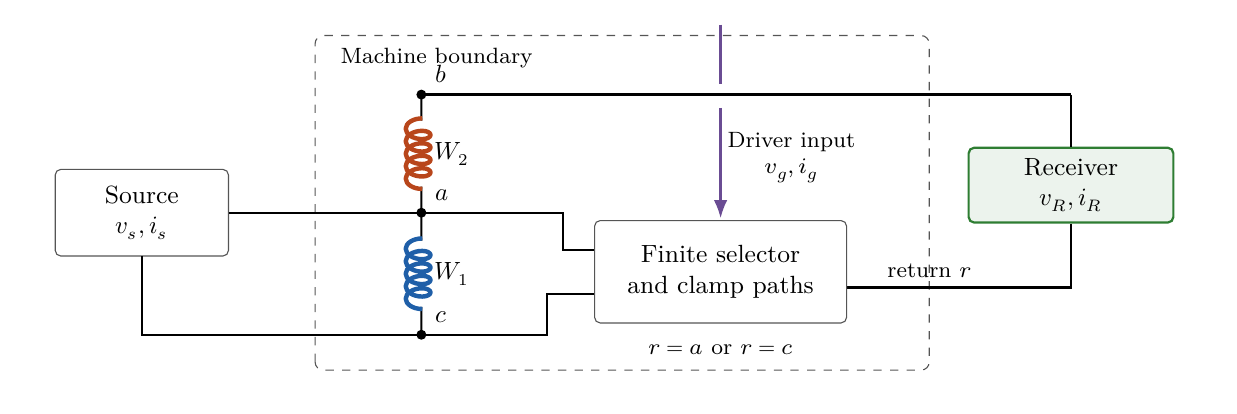
\begin{tikzpicture}
\path[use as bounding box] (0,-.65) rectangle (15,3.9);
\draw[boundary] (3.65,-.45) rectangle (11.45,3.8);
\node[font=\footnotesize,anchor=north west] at (3.85,3.77) {Machine boundary};
\node[block,minimum width=2.2cm,minimum height=1.1cm] (src) at (1.45,1.55) {Source\\$v_s,i_s$};
\draw[thick] (src.east)--(5,1.55);
\draw[thick] (1.45,1.0)--(1.45,.0)--(5,.0);
\draw[thick] (5,.0) to[L,l_=$W_1$,color=elemA] (5,1.55)
 to[L,l_=$W_2$,color=elemB] (5,3.05);
\foreach \y/\n in {0/c,1.55/a,3.05/b} {
 \fill (5,\y) circle(1.8pt);
 \node[anchor=south west] at (5.05,\y+.03) {$\n$};
}
\draw[thick] (5,3.05)--(13.25,3.05);
\node[block,receiver,minimum width=2.6cm,minimum height=.95cm] (rec) at (13.25,1.9) {Receiver\\$v_R,i_R$};
\draw[thick] (13.25,3.05)--(rec.north);
\draw[thick] (rec.south)--(13.25,.6)--(10.4,.6);
\node[block,minimum width=3.2cm,minimum height=1.3cm] (sw) at (8.8,.8)
 {Finite selector\\and clamp paths};
\draw[thick] (5,1.55)--(6.8,1.55)--(6.8,1.08)--(sw.west |- 0,1.08);
\draw[thick] (5,0)--(6.6,0)--(6.6,.52)--(sw.west |- 0,.52);
\node[font=\footnotesize,above] at (11.45,.6) {return $r$};
\node[font=\footnotesize] at (8.8,-.19) {$r=a$ or $r=c$};
\node[font=\footnotesize,align=center] at (9.7,2.25) {Driver input\\$v_g,i_g$};
\draw[elemD,thick] (8.8,3.94)--(8.8,3.18);
\draw[flow,elemD] (8.8,2.88)--(8.8,1.48);
\end{tikzpicture}
\end{document}
